\chapter{Estado del arte}

%Introduccion que unifique creación del espectáculo con obtención de la geometría.%
%Si NO es posible unificarlos explicar de todas maneras que estas dos cosas se estudian como temas disjuntos, y como convivirían.%
%Estas dos cosas por más que sean disjuntas se unen en la solución del proyecto.%

\section{Creación de un espectáculo de \emph{video mapping}}

El proceso de creación de un espectáculo de \emph{video mapping} se analiza en este proyecto, dividiéndolo en tres etapas que son el modelado de la escena, la producción del espectáculo y la proyección del mismo.
Esta división se apoya en el estudio del estado del arte que incluye entrevistas a \emph{VJs} anexadas en \titleref{chapter:aportes}.

En el modelado de la escena se obtiene una representación virtual y abstracta de los objetos reales sobre los que se proyectará.
Este modelo será la base para trabajar en posteriores etapas y sobre el cuál se diseñará el espectáculo.

En la siguiente etapa se realiza la producción del espectáculo que consiste en definir los distintos efectos visuales a ser aplicados sobre los objetos modelados.
La reproducción de estos efectos podrá ser orquestada en el caso que el espectáculo sea una visualización de efectos predefinida, como las que se ven en presentaciones sobre fachadas y lanzamiento de productos.
También un espectáculo podrá ser dinámico, en el cuál, un \emph{VJ} decidirá en tiempo real los efectos a desplegar.
En este caso no se realiza una orquestación de los efectos en esta etapa, sino que se define una interfaz para que el \emph{VJ} ejecute de forma simple el efecto deseado.
Esto puede ser, por ejemplo, definiendo una tecla para cada efecto a mostrar.
En esta etapa también se diseña y produce la musicalización que será utilizada durante todo el espectáculo.

Es en la proyección del espectáculo en donde se puede contemplar el resultado de los distintos efectos visuales proyectados sobre las superficies acompañados por efectos de sonido.
Para lograr la correspondencia en la proyección de los objetos del modelo con las superficies se debe calibrar la proyección.
Esta correspondencia se logra modificando el modelo de la escena, ajustando la posición y orientación de los proyectores, y ajustando los parámetros intrínsecos$^\dagger$ de la proyección.
%Esta etapa no es necesariamente una proyeccion final sino que se puede simular%

Cada una de estas etapas será abordada en esta sección desde dos enfoques diferentes: bidimensional y tridimensional.
% 
% 
% 
% 
% 

%Las distintas herramientas actuales para realizar espectáculos de \emph{video mapping} optan por uno de estos dos enfoques para abordar el problema.
%

%explicacion de pie de diagrama:redactarlo mejor, El modelo generado en 2d depende del punto de vista del proyector y puede no parecerse a la realidad.
%El modelo generado 3d se asimila a la realidad y luego con la cámara virtual ajusto el punto de vista del proyector.

\begin{figure}[H]
  \centering
    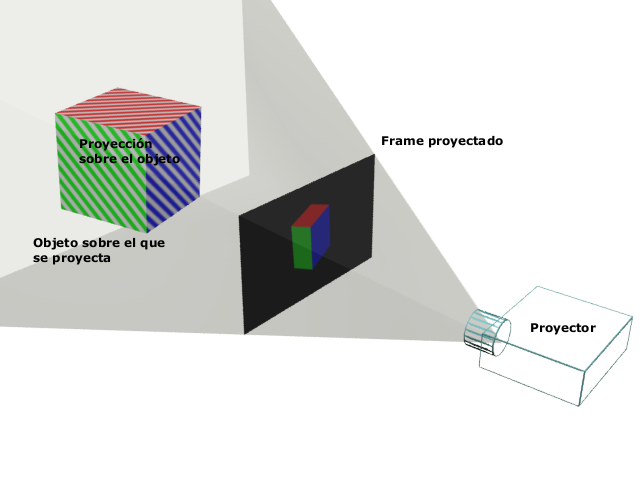
\includegraphics[width=0.7\textwidth]{./Cap2_videomapping/proy2dvs3d}
  \caption[Imagen propia]{Esquema de proyección.}
  \label{fig:proy2dvs3d}
\end{figure}

\subsection{Enfoque bidimensional}
\subsubsection{Modelo}
Un modelo bidimensional refleja lo que vería un observador desde un punto de vista fijo.
%si se quieren agregar hay en el SVN imagenes de proyeccion perspectiva y paralela  VER
Técnicamente es el resultado de una proyección en perspectiva \cite{LibroCompGrafica} sobre un plano de vista de los elementos de la superficie a modelar.

Este punto de vista debe ser considerado al posicionar y orientar el proyector que reproducirá el espectáculo.
La posición, orientación y campo de vista del proyector definirán además la sección de superficie sobre la que se proyectará.
En caso de utilizar más de un proyector cada uno de estos será posicionado en un lugar diferente y por lo tanto será necesario un modelo por cada uno de ellos.

\begin{figure}[H]
  \centering
    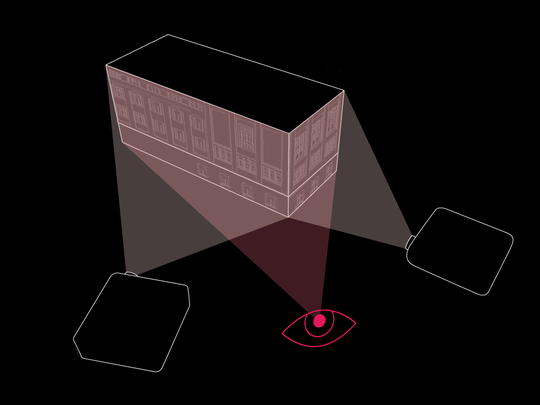
\includegraphics[width=0.7\textwidth]{./Cap2_videomapping/diagrama-2proyectores}
  \caption{Proyectores y sus puntos de vista.}% vvvv.org/ %
  \label{fig:diagrama-2proyectores}
\end{figure}

Son ejemplos de modelos una fotografía, un plano arquitectónico de una fachada o figuras geométricas bidimensionales que representan las secciones de las superficies.
En algunos casos estos se combinan para obtener como resultado un único modelo.
\begin{itemize}
  \item Una fotografía. Ubicando la cámara de forma que su punto de vista y el del proyector coincidan minimizará los ajustes necesarios en la etapa de calibración.%extender y que no quede tan en el aire lo de ajustes de calibracion%
  \item Un plano arquitectónico contiene información exacta de las medidas de la superficie que representa en una escala dada. Generalmente utiliza el método de proyecciones paralelas \cite{LibroCompGrafica} sobre un plano de proyección. Para utilizar el plano arquitectónico como modelo se debe transformar de forma que coincida con la proyección en perspectiva desde el punto vista que estará ubicado el proyector.
  \item Las figuras geométricas modelan sectores de la superficie donde se proyectará. Un método para generar las figuras geométricas consiste en utilizar un proyector y herramientas de software que permiten delinear el contorno de las secciones de la superficie en tiempo real. Se observa el resultado de cada figura generada proyectada sobre la superficie ajustando el modelo en el momento de la construcción.%%%figuras geometricas queda muy abstracto, hay que llevarlo mas al tema de representacion digital de quads%%%
\begin{figure}[H]
  \centering
    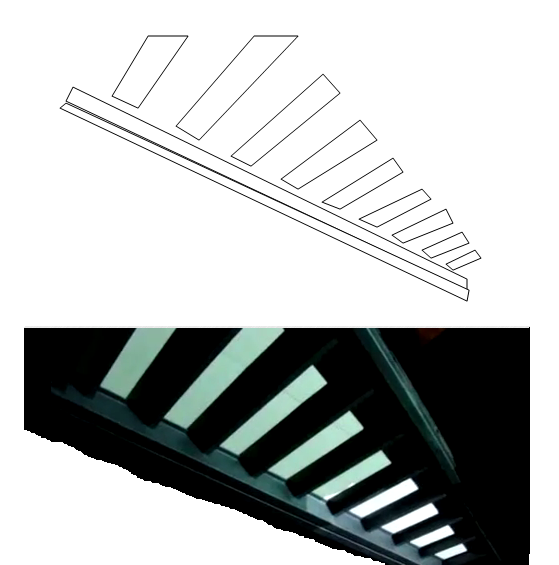
\includegraphics[width=0.7\textwidth]{./Cap2_videomapping/RepresentacionconfigurasGeometricas}
  \caption{Representación con figuras geométricas.}%imagen nuestra no necesita referencia%
  \label{fig:RepresentacionconfigurasGeometricas}
\end{figure}

Al usar el proyector para obtener el modelo queda incorporada la perspectiva del mismo y si no se modifica su posición y orientación no sería necesaria otra calibración.
Otra opción es dibujar las figuras con una fotografía o plano de fondo. En este caso la construcción de las figuras geométricas se realiza delineando el contorno de la superficie en la fotografía o plano.
Una forma automática de generar el modelo es utilizando técnicas de visión por computadora$^\dagger$, por ejemplo, en base a algoritmos de reconocimiento de aristas \cite{ArticuloAutom2dmodel}.
\end{itemize}

\subsubsection{Producción del espectáculo}
La producción del espectáculo en dos dimensiones consiste en definir efectos visuales sobre regiones de un espacio bidimensional discreto$^\dagger$ representadas en el modelo de la escena. Este espacio bidimensional discreto se representa con coordenadas de pantalla que identifican cada uno de los píxeles$^\dagger$ del área de trabajo. Los efectos visuales se logran realizando cualquier animación computacional que genere una salida gráfica como pueden ser videos e imágenes.
En esta etapa, además de definir los efectos, se planifica en qué momento se mostrarán cada uno de ellos, pudiendo sincronizarse con la música que forma parte del espectáculo.
%Mencionar caso de espectaculos en vivo%

En computación gráfica se utilizan texturas para proyectar videos e imágenes sobre regiones del área de trabajo. Las texturas son mapas de bits$^\dagger$ utilizados para cubrir la superficie de un objeto virtual. Estos mapas de bits pueden ser generados a partir de imágenes, videos, o incluso dinámicamente mediante algoritmos permitiendo así crear efectos visuales como, por ejemplo, la transición de un color a otro.
Cuando se utilizan videos estos pueden ser generados teniendo en cuenta la superficie donde se está proyectando y el punto de vista desde donde se contemplará el espectáculo. Esto es particularmente importante cuando el contenido a mostrar pretende crear una ilusión tridimensional, pues la perspectiva debe coincidir con la de los espectadores.%ampliar o explicar mejor%
\begin{figure}[H]
  \centering
    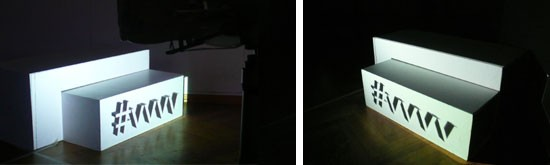
\includegraphics[width=0.7\textwidth]{./Cap2_videomapping/3dillusion}
  \caption{Izq. Ilusión 3D lograda. Der. No se logra la ilusión.}% vvvv.org/ %
  \label{fig:3dillusion}
\end{figure}

En este contexto se habla de mapeo, no como la salida a través de un equipo proyector, sino como la operación que logra una correspondencia entre una textura y una figura geométrica que no necesariamente coinciden en tamaño y forma. Para esto se definen coordenadas de textura en cada vértice de la figura geométrica que referencian distintas ubicaciones dentro de la misma.
Las coordenadas de las texturas tienen dos componentes: una horizontal y una vertical llamadas U y V. Si el valor de estas componentes se normaliza entre 0 y 1 entonces la esquina superior izquierda de la textura se corresponderá con la coordenada (0,0), la superior derecha con (1,0), la inferior izquierda con (0,1) y la inferior derecha con (1,1).
%agregar referencia a correspondencia de textura en un objeto, ver para imagen http://en.wikipedia.org/wiki/UV_mapping
Los vértices de una figura geométrica se asocian con coordenadas UV que definen el punto de la textura que se corresponde sobre el vértice. Mediante interpolación se logra mapear toda la textura a la figura geométrica.
Si bien es posible mapear una textura a cualquier figura geométrica, esta correspondencia es más directa utilizando un cuadrilátero ya que a cada uno de los vértices se lo hace corresponder con una esquina de la textura. A su vez el cuadrilátero es la figura básica en las aplicaciones\footnote{Las aplicaciones relevadas utilizan el cuadrilátero como figura básica. Ver apéndice: Aplicaciones relevadas.} de \emph{video mapping}.
Estos cuadriláteros se utilizan como piezas constructoras del espectáculo, cubriendo sectores del modelo sobre los cuales luego se aplican las texturas permitiendo crear los distintos efectos visuales.

\subsubsection{Calibración}
La calibración se utiliza para ajustar el modelo con la superficie que representa. Inicialmente se fija la posición y orientación del proyector y luego, con ayuda de herramientas de software, se aplica la transformación geométrica homografía\footnote{Ver sección: Obtención de geometría} a la proyección resultante, para lograr la correspondencia.
En caso de haber modificaciones en la posición y orientación del proyector la calibración deberá realizase nuevamente. %reescribir esta oración%

Los ajustes necesarios varían dependiendo del método utilizado para obtener el modelo. En caso de utilizar una fotografía, el proyector deberá ser ubicado de forma tal que el punto de vista de la cámara con la que se tomó coincida con el del proyector y así lograr la coincidencia del centro de proyección. Igualmente son necesarios ajustes ya que los lentes de la cámara y el proyector no necesariamente coinciden en el ángulo de visión \cite{LibroCompGrafica2}\cite{LibroPhotographicOptics}. Con el método de generación de figuras geométricas, en el que se modelan las secciones de la superficie a mapear utilizando el mismo proyector, los ajustes se reducen a lograr la misma posición y orientación que tenía el proyector al momento de la captura de secciones, ya que las deformaciones relacionadas a los parámetros intrínsecos fueron implícitamente consideradas durante el proceso de captura.

\subsection{Enfoque tridimensional}
\subsubsection{Modelo}
Para el modelado tridimensional se pueden utilizar representaciones de cuerpos y superficies tridimensionales representadas por mallas$^\dagger$ de polígonos \cite{Mesh_building}, comúnmente utilizadas en disciplinas como cartografía, visión computacional y computación gráfica. A diferencia de un modelo bidimensional, éste no depende de un punto de vista, lo que permite al diseñador visualizar la escena desde diferentes ángulos. Las entidades que conforman la malla son vértices, aristas, caras y atributos numéricos que representan la posición y normales de los vértices, coordenadas de textura y colores. La topología de la malla puede variar, por ejemplo, los polígonos que la componen pueden tener distinta cantidad de vértices.

\begin{minipage}{0.35\textwidth}
\begin{flushleft} \large
\begin{figure}[H]
  \centering
    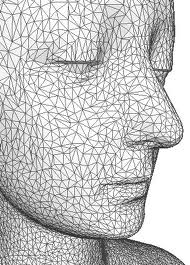
\includegraphics[width=0.7\textwidth]{./Cap2_videomapping/EjemploMallaTriangular}
  \caption{Mallas triangulares.}%ref  http://stochastix.wordpress.com/2008/07/15/bust-of-mystery/ %
  \label{fig:mallas1}
\end{figure}
\end{flushleft}
\end{minipage}
\begin{minipage}{0.45\textwidth}
\begin{flushright} \large
\begin{figure}[H]
  \centering
    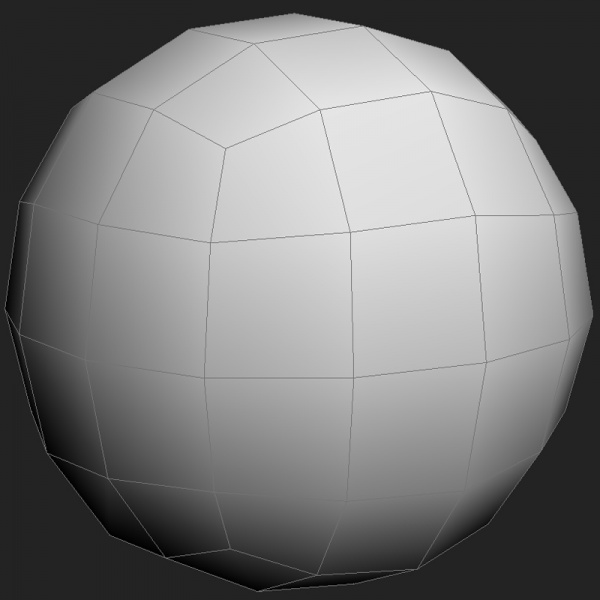
\includegraphics[width=0.75\textwidth]{./Cap2_videomapping/EjemploMalla4Vertices}
  \caption{Mallas de cuadriláteros.}%ref  http://www.fallingpixel.com/perfect-sphere-mesh-384-polygons-3d-model/35623  %
  \label{fig:mallas2}
\end{figure}

\end{flushright}
\end{minipage}

Existen técnicas como la de \emph{remeshing} que mediante la utilización de algoritmos específicos reducen la cantidad de vértices de la malla sin perder la representatividad de la superficie, logrando así un manejo más performante de las mallas. %Ampliar el uso de estas tecnicas de remeshing%
%si se quiere se pone esta referencia:Survey of Polygonal Surface Simplification Algorithms Paul S. Heckbert and Michael Garland doc/papers/Mesh_building/Survey of Polygonal Surface Simplification Algorithms.pdf

Los modelos tridimensionales se generan utilizando distintas técnicas:
\begin{itemize}
  \item Modelado utilizando polígonos: a partir de mallas que representan figuras primitivas se podrán construir nuevas mallas, por ejemplo aplicando operaciones de unión o resta.
  %Que es union y resta?, explicar esto o algo mas general, union y resta son solo dos ejemplos y no los mas representativos%
  También se aplican transformaciones que modifican las aristas, vértices o caras, aproximando el resultado a la superficie que se desea modelar.
  \item  Modelado utilizando curvas: a partir de una jaula creada por curvas se aplican transformaciones para modificarla, manipulando sus puntos de control. Es utilizado en modelado de automóviles, edificios y mobiliario, entre otros.
  %programas: Maya, 3D Studio Max
  \item Esculpido digital: técnica digital que simula el esculpido convencional, en la que software especializado provee una interfaz para modificar el modelo de forma detallada, oprimiendo y resaltando zonas de la superficie. Es utilizado para lograr efectos especiales en video juegos y películas logrando figuras y texturas complejas, entre otras.
  %programas: 3D-Coat, Zbrush, y Mudbox
  \item Reconstrucción a partir de fotografías: se obtiene la representación de la superficie mediante mediciones de los objetos fotografiados. Conociendo la escala de la imagen se extrapola y se obtiene la distancia entre dos puntos en la superficie. Es usada en arquitectura, ingeniería, geología, arqueología, etc.
  %esta técnica es llamada fotogrametría en dos dimensiones, estereofotogrametría para obtener información tridimensional
  \item Reconstrucción utilizando hardware especializado: utilizando escáneres tridimensionales se obtiene una nube de puntos$^\dagger$ que representa la superficie. Generalmente la cantidad de información obtenida es densa provocando redundancia. Es por esto que se utilizan algoritmos especializados para reducir la nube de puntos.
  %explicar que el ruido tambien genera informacion que se debe depurar%
  %se puede poner una nota al pie, que esta técnica se ampliará en el capítulo Reconstrucción

\end{itemize}
\subsubsection{Producción del espectáculo}
La producción del espectáculo en tres dimensiones agrega un nivel de abstracción adicional a la producción bidimensional. Esto permite que el diseñador cree un espectáculo transformando directamente los objetos del modelo tridimensional y no sus perspectivas como en el anterior enfoque.
Esto plantea un cambio en la forma de trabajar en el espectáculo y de planificar la producción, ya que el diseñador no estará restringido a considerar ubicación alguna de los proyectores. Esta preocupación se traslada a etapas posteriores.

El modo de trabajo se basa en mapear texturas sobre las caras de los objetos tridimensionales de forma análoga a como se realiza sobre figuras bidimensionales. En este tipo de modelos podría ser deseable mapear una textura de forma que abarque varias caras del mismo objeto tridimensional, por ejemplo, la superficie de un cilindro. Para lograrlo se deben mapear distintos sectores de la textura en cada una de las caras que conforman la superficie, utilizando coordenadas de textura en cada uno de los vértices. La diferencia está en que en este enfoque los vértices no se encuentran necesariamente en el mismo plano, por lo que ajustar una textura bidimensional a este tipo de superficies no es tan directo. Para ello existen técnicas que asisten en la tarea de definir las coordenadas de textura. Una de ellas consiste en aproximar la superficie por una primitiva conocida más simple como puede ser un cubo, cilindro, esfera o plano. Para estas superficies existen funciones matemáticas que proyectan cada punto de la superficie a un plano. De esta forma se pueden determinar las coordenadas $UV$. Un ejemplo de esto para esferas son las proyecciones utilizadas para representar el planisferio como la proyección cilíndrica equidistante \cite{flatteningTheEarth}. Otra técnica es $UV$ \emph{unwrapping} que consiste en desenvolver los vértices de la superficie, aplanándolos sobre la textura. De esta forma el mapeo se realiza de forma más intuitiva ya que la superficie aplanada es bidimensional al igual que la textura. Esta técnica es soportada por la mayoría de los programas de edición de gráficos tridimensionales que proveen distintas herramientas para ajustar la forma en que se desenvuelve la textura.

En la escena tridimensional los objetos son visualizados utilizando cámaras virtuales que fijan un punto de vista. En la salida gráfica se representará entonces la escena desde la perspectiva de una cámara virtual, permitiendo visualizarla desde distintos ángulos. Esto posibilita definir el punto de vista del proyector que reproducirá la salida gráfica, y no se restringe a realizarlo antes de producir el espectáculo sino que una vez producido es posible observar el resultado y elegir el punto de vista que más agrade.
Producir el espectáculo transformando directamente los objetos y no sus perspectivas permite escalar con mayor facilidad en la cantidad de proyectores. Lo único que habría que agregar serían cámaras virtuales que definan más puntos de vista sin modificar el modelo ni los efectos producidos.

Si bien se está abordando un enfoque tridimensional de la producción del espectáculo, existen casos en que es más sencilla la implementación de ciertos efectos tomando un enfoque en dos dimensiones, sobre todo cuando estos se aplican sobre regiones planas de la superficie. Es por esto que es muy común combinar ambos enfoques y utilizarlos de acuerdo a las necesidades del diseñador. Cabe aclarar que al combinar los enfoques se pierden las ventajas de definir el punto de vista del proyector luego de la producción por lo que los objetos bidimensionales y efectos sobre estos se deben definir una vez fijada la ubicación de los proyectores.

\subsubsection{Calibración}
%Hablar de forma genérica de la calibración%

%Redondear el tema de ENFOQUE 2D y 3D luego de hablar de las 3 etapas%

\section{Obtención de geometría}

En este capítulo se presenta la reconstrucción tridimensional automática de una superficie utilizando técnicas computacionales.
Se introducen distintos métodos que permiten la construcción automática de modelos, discutiendo sus características según propiedades de la superficie a representar y tecnologías utilizadas.
La construcción del modelo se presenta en dos etapas. Inicialmente se obtiene una nube de puntos correspondiente a la superficie utilizando técnicas y dispositivos para este propósito, para luego procesar la información obtenida y construir una malla tridimensional. Mediante este procesamiento se obtienen propiedades adicionales como grupos de puntos que representan caras de una malla y las normales que identifican la orientación de la superficie.

\subsection{Obtención de la nube de puntos}

En esta sección se estudian los fundamentos matemáticos, técnicas y dispositivos relacionados al problema de la correspondencia de puntos de la realidad con puntos bidimensionales en el plano imagen, obtenido por una cámara, y la posterior determinación de su profundidad. 

\subsubsection{Correspondencia}

\subsubsection{Visión estéreo}

\cite {StereoReview} El análisis de imágenes de video en estéreo se ha utilizado como método para reconstruir la estructura tridimensional de una escena, este método no utiliza luz auxilar, por esta razón es un método pasivo. El análisis de las imágenes se realiza por medio de algoritmos que han evolucionado en los últimos tiempos logrando la reconstrucción de escenas rápidamente, es por esto que esta técnica es muy utilizada en implementaciones que necesitan respuesta en tiempo real.
En la reconstrucción utilizando el modelo de cámara estéreo se identifican dos pasos a seguir, primero resolver el problema de la correspondencia, esto es dadas dos imágenes de la escena para todos los puntos de una imagen se obtiene el punto correspondiente en la otra imagen y se calcula la desigualdad de cada punto, es decir la distancia en \emph{pixels} entre los puntos que se corresponden.
Y segundo resolver el problema de triangulación\footnote{ver anexo de método de triangulación}, teniendo en cuenta la desigualdad definida en la correspondencia utilizando el método de triangulación se obtiene la distancia focal de cada punto a cada una de las cámaras, de esta forma se calcula la profundidad del punto.
\begin{figure}[H]
  \centering
    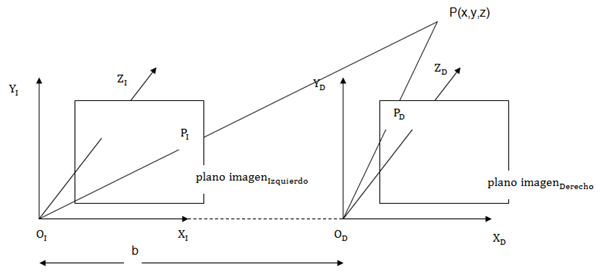
\includegraphics[width=0.5\textwidth]{./Cap2_videomapping/stereo.PNG}
  \caption{geometía estéreo con ejes paralelos}%Structure from Stereo- A Review  Umesh R. Dhond and J.K.Aggarwal 1989%
  \label{fig:Stereo}
\end{figure}
Un caso simple sería con los ejes ópticos de las cámaras paralelos y los planos de imagen coplanares, como se muestra en la figura, en este caso las líneas epipolares\footnote{ver anexo de geometría epipolar} correspden a las filas en el \emph{frame buffer} y la correspondencia de los puntos es buscada en esas filas.
\begin{figure}[H]
  \centering
    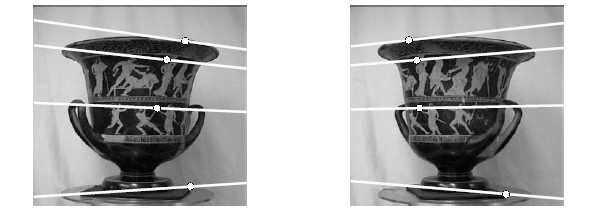
\includegraphics[width=0.5\textwidth]{./Cap2_videomapping/epipolar3.PNG}
  \caption{dos imágenes con las líneas epipolares y puntos que se corresponden}%Geometía de Cámaras  StereoReview pag 241. fig 9.3%
  \label{fig:Stereo2}
\end{figure}

En los casos más comunes no se tienen estas características, y por ello es necesario introducir parámetros en los cálculos que hacen el ajuste del modelo ideal, modelo \emph{pinhole} al modelo de las cámaras reales. 

Existen variedad de algorimos que solucionan el problema de correspondecia y cálculo de desigualdad entre los puntos de las dos imágenes se clasifican según diferencias en las imágenes destacándose dos estrategias:
\begin{itemize}
   \item \emph{separate area}: basada en correlación del brillo e intensidad. Se utilizan patrones de brillo aplicados a un píxel y sus vecinos utilizando principio de localidad. Las diferencias en la perspectiva de la imagen o cambios en luminosidad absoluta de la escena pueden generar errores.
   \item \emph{features}: las características usadas para la correspondencia son aristas, puntos o segmentos dadas por cambios de intensidad de la imagen. Esta estrategia es más estable ante la variación de luminosidad absoluta y en la práctica la correspondencia es más rápida.
\end{itemize}
La principal desventaja de este método es que en caso de oclusión, hay regiones que no tienen correspondencia en las dos imágenes por esto no se puede resolver el problema de correspondencia para estas regiones.

\subsubsection{Luz estructurada}

Un método basado en la técnica de luz estructurada consiste en un sistema formado por una o mas cámaras de video mas un proyector que despliega distintos patrones sobre la superficie a modelar. Los patrones son capturadas por la o las cámara de video para su posterior analisis. Mediante patrones codificados apropiadamente para la escena observada, se resuelve el problema de correspondencia de los puntos de la escena con los capturados, y luego, mediante un análisis de las deformaciones de los patrones se obtiene información tridimensional de la posición, orientación y textura de la superficie\cite{SLightPatterns}.

\paragraph{Clasificación de patrones}

Los sistemas que utilizan luz estructurada se basan en la proyeccion de un patron o secuencia de patrones que identifican cada uno de los \emph{pixeles} en la región iluminada mediante una palabra clave. 
La figura XXX muestra la clasificacion de patrones propuesta en \cite{SLightClassification} en la que se diferencian principalmente por la naturaleza continua o discreta de los mismos. 

%figura de patrones clasificados%
\begin{figure}[H]
  \centering
    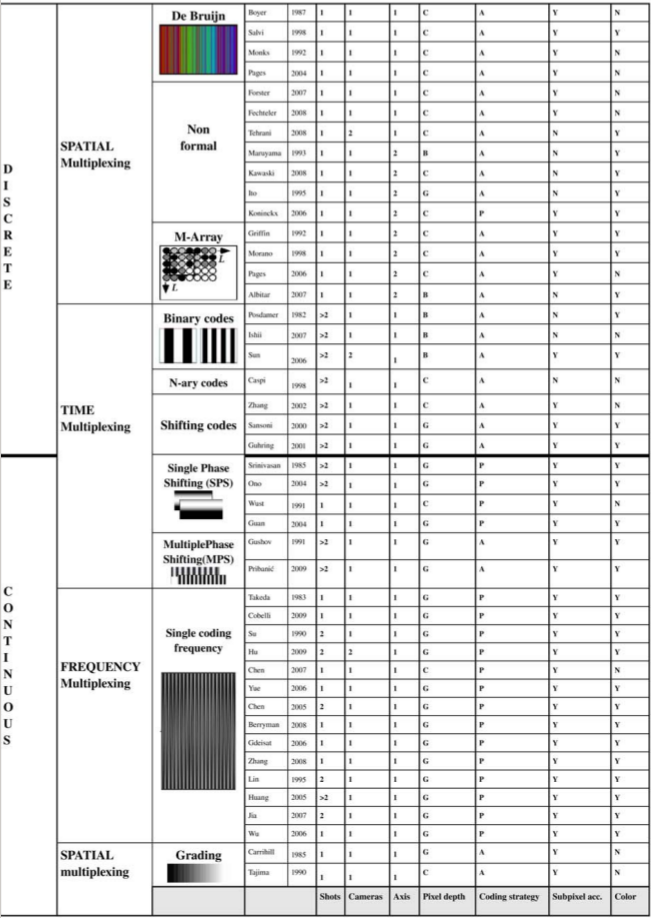
\includegraphics[width=0.8\textwidth]{./Cap2_videomapping/SL-patternclassiff.png}
  \caption{Clasificación de patrones de luz estructurada \cite{SLightClassification}}
  \label{fig:SLPatternClassification}
\end{figure}

Los patrones discretos asignan el mismo valor a todos los puntos de la región representada por la misma codificación, mientras que los continuos utilizan una representación más suavizada en donde cada \emph{pixel} tiene una codificación unica dentro de la región, variándose la intensidad o el color a lo largo de uno o ambos ejes en la proyección.

Las tecnicas mas comunes utilizan codificacion binaria \footnote{binary code}, que consiste en proyectar en una mitad de la pantalla una columna en blanco y en la otra mitad negro y determinar si un punto siendo observado aparece como blanco o negro. Esto determina de que lado de la escena se encuentra dicho punto. Realizando la misma division en la región de la escena donde se espera que el punto se encuentre, es posible determinar la coordenada en $X$ de dicho punto. Este proceso funciona como una busqueda binaria tradicional, por lo tanto toma log2(w) subdivisiones el encontrar la posicion exacta del punto. A modo de ejemplo, para un proyector con una resolucion de 1024x768 \emph{pixeles} son necesarias log2(1024)=10 subdivisiones. Otra forma de codificación binaria que obtiene mejores resultados es la llamada \emph{gray code}. El primer paso de la subdivision es similar en cuanto a que divide la mitad izquierda y derecha del area en blanco y negro. Los siguientes patrones proyectados son diferentes con la particularidad que dos columnas adyacentes del patrón difieren solamente en un bit. Esto ultimo implica menos errores al momento de decodificar puntos cercanos a las fronteras.  

La codificación \emph{gray code} tiene la desventaja de la cantidad de marcos que se necesitan para el procesamiento (10 \emph{frames}). Un metodo que mejora este aspecto es el llamado \emph{Three Phase-Shifting} que utiliza tres ondas sinusoidales para la determinacion de columnas. El metodo es explicado en detalle en \cite{3DShapeMeasurement} y \cite{SLThreeStepPhaseShift} por Zhang e implementado por Kyle McDonalds en \cite{KyleMcDonald}. Una desventaja de este algoritmo, y por tanto tambien de la implementacion de \emph{Structured Light} de Kyle, es que obtiene buenos resultados solo al escanear superficies mas o menos continuas.

\paragraph{Calibración}

En esta sección se describe un método originalmente propuesto por Zhang [Zha00] para la calibración de una cámara y un proyector con el objetivo de capturar correctamente los patrones proyectados para su posterior análisis. 

La calibración de la cámara requiere estimar inicialmente los parámetros del modelo de cámara pinhole. Por lo tanto se deberán obtener los parámetros intrínsicos como distancia focal, punto principal y factores de escala, y los extrínsicos definidos por la matriz de rotación y vector de traslación de un punto en el espacio al sistema de coordenadas de la cámara. 
%We recommend the reader review [HZ04, MSKS05] for an in-depth description of camera models and calibration methods
%el modelo pinhole que nosotros presentamos no incluye los extrinsicos (matrices de traslacion y rotacion) 

Básicamente la calibracion de la cámara requiere la captura de una secuencia de imagenes de un objeto simple, con un conjunto de caracteristicas fijo y distinguibles, y con un desplazamiento tridimensional conocido. Esto permite que cada imagen capturada durante el proceso de calibracion provea de un conjunto de correspondencias de los puntos tridimensionales de la escena a puntos bidimensionales en el sistema de coordenadas de la camara. Particularmente, en el método de Zhang, el objeto conocido que se observa es un tablero de damas plano en una o mas orientaciones. De la secuencia capturada se pueden obtener los parametros intrinsicos y luego, utilizando una sola toma de la secuencia,  se obtienen los parametros extrinsicos.

Para la calibracion del proyector, este se modela como el inverso de una cámara, teniendo en cuenta que la luz viaja en la dirección opuesta y que un punto en el plano de la imagen se mapea a un rayo de luz saliente por el punto y por el centro de proyeccion. Dado este modelo, la calibración sucede de forma similar a la de una cámara, pero en lugar de tomar imágenes de un tablero de damas fijo, se proyecta un tablero en una ubicacion conocida y se toman imagenes del mismo utilizando la cámara para analizar las distorsiones. Este enfoque resulta ser una extension directa del metodo de Zhang para calibración de cámaras, por lo que toda la teoria y software disponible es reutilizado.

Existen varias implementaciones de esta tecnica de calibracion basado en el modelo inverso de la cámara, la mayoria de ellos desarrollados por investigadores para uso propio. Puede observarse una de estas implemtaciones, BYO3D\cite{BYO3D}, en la que se proveen dos alternativeas, un \emph{Toolbox} de MATLAB\cite{MATLAB} y una extension a la biblioteca de visión computacional\footnote{computer vision} OpenCV\cite{OpenCV}.

\subsubsection{Kinect}

\emph{Kinect} es un dispositivo que se puede adicionar a la consola \emph{Xbox360} de \emph{Microsoft}. El objetivo de este dispositivo es permitir que el usuario interactúe con la consola utilizando solo el movimiento de su cuerpo. Para lograr esto, \emph{Kinect} aplica distintas técnicas de procesamiento de imágenes, considerando ubicaciones, posturas y distancias. El \emph{hardware} de \emph{Kinect} no consiste tan solo de una cámara, sino que tiene adicionalmente un emisor de infrarrojos que en base a la deformación del haz de luz determina la distancia de cada punto de la imagen capturada. Posteriormente, combina la información visual para tener una noción bastante precisa de los movimientos del usuario. A mediados del 2011 fue presentada una interfaz de programación gratuita que permite utilizar \emph{Kinect} de forma directa en aplicaciones no licenciadas para diferentes propósitos, no solo el de los videojuegos.

\begin{figure}[H]
  \centering
    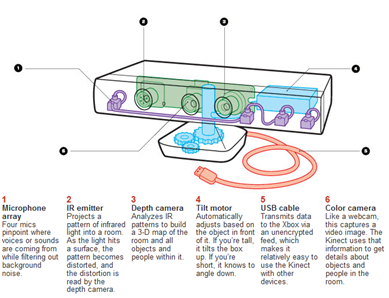
\includegraphics[width=0.7\textwidth]{./Cap2_videomapping/kinect.PNG}
  \caption{Componentes de un sensor Kinect}%ref  paper http://events.ccc.de/congress/2011/Fahrplan/attachments/1969\_kinectfusion-uist-comp.pdf  ? %
  \label{fig:Kinect}
\end{figure}

Para el análisis de las deformaciones de los rayos y construir el mapa de profundidad, \emph{Kinect} utiliza la previamente mencionada técnica de luz estructurada. Mediante el emisor infrarrojo con el que viene equipado, se proyectan los patrones de luz por toda la escena y utilizando la cámara de profundidad se analizan las distorsiones.
También se cuenta con una cámara convencional para analizar objetos o personas en la escena y la detección de colores.
En cuanto a los usos específicos orientados a la reconstrucción tridimensional de objetos, el proyecto \emph{KinectFusion} \cite{KinectFusion}, actualmente patrocinado por \emph{Microsoft}, logra muy buenos resultados.%extender kinectfusion%

\subsection{Procesamiento de nube de puntos}

Al utilizar técnicas de obtención de geometría lo que se obtiene son nubes de puntos. Es necesario simplificar este modelo con el objetivo de eliminar redundancia y aumentar la velocidad en el procesamiento de los datos. Un problema adicional al volumen de la información obtenida es que comúnmente se introduce ruido. Para solucionar este problema se realiza un suavizado en el procesamiento de la nube de puntos \cite{PCloudSimplify}.

Las heurísticas existentes para reducir nubes de puntos pueden clasificarse en tres grandes grupos \cite{PntCloud}:
\begin{itemize}
   \item \emph{Clustering methods}: consiste en obtener grupos de la nube de puntos en donde cada grupo se remplaza por un conjunto de puntos representativos en él. Los grupos se pueden construir utilizando un enfoque incremental en el cual estos son creados iniciando por un punto aleatorio y agregando puntos vecinos hasta llegar a una cantidad establecida de elementos o un enfoque jerárquico en donde se particiona el conjunto de puntos recursivamente hasta conseguir grupos de un tamaño predefinido.
   \item \emph{Iterative simplification}: se recorren iterativamente los puntos de la nube contrayendo parejas en un único punto. Se evalúa el error introducido, utilizando mínimos cuadrados, que se genera en la contracción comparándolo con el error que se obtendría al contraerse con otro punto vecino eligiendo la contracción que introduce menor error al sistema. La simplificación se da por finalizada por haber logrado la cantidad de puntos deseada o por superar una cota de error a introducir en el sistema.
   \item \emph{Particle simulation}: se generan nuevos puntos que sustituyen la nube de puntos original. Se generan conjuntos de partículas que se mueven aleatoriamente en la superficie hasta lograr un balance. %Luego, utilizando el algoritmo de point–repulsion se definen en las zonas que hay mayor colisiones.%
\end{itemize}

Luego de simplificar la nube de puntos se construye un modelo tridimensional a partir de ella utilizando mallas de triángulos. La razón principal es la simplicidad de los algoritmos que dibujan triángulos. Esto permite que sean implementados fácilmente en hardware además del beneficio de que cualquier polígono con más de tres caras puede representarse como un conjunto de triángulos \cite{PCloudTriangle}.

A continuacion se detallan los algoritmos asociados a cada paso de un típico procesamiento de malla que toma como entrada una nube de puntos, realiza un sub-muestreo y suavizado de la misma, calcula las normales en cada punto de la nube y finalmente aplica algoritmos de reconstrucción de la malla. Esto ha sido estudiado e implementado en bibliotecas como \emph{VcgLib} \cite{VCGLib} y \emph{CGAL} \cite{CGAL}, pero lo presentado se corresponde con la implementación de \emph{VcgLib}. 

\begin{figure}[H]
  \centering
    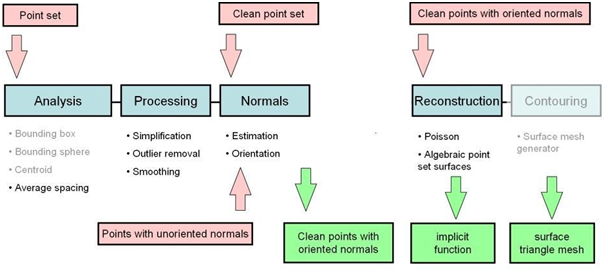
\includegraphics[width=0.5\textwidth]{./Cap2_videomapping/malla-flow.png}
  \caption{Flujo típico de procesamiento de nubes de puntos \cite{CGAL}}
  \label{fig:Mesh-CGAL}
\end{figure}

\subsubsection{Muestreo \emph{Poisson-disk}}

%falta referencia%
El muestreo de variables aleatorias es una técnica utilizada para una gran variedad de aplicaciones como procesamiento de imágenes y geometrías. Particularmente, el muestreo \emph{Poisson-disk} se utiliza para la ubicación aleatoria de objetos en mundos artificiales, algoritmos de texturas procedurales y procesamiento de geometrías o mallas.%REFERENCIAR%
Esta técnica genera conjuntos de puntos con la propiedad de obtener puntos suficientemente juntos pero con la restricción de no estar más próximos unos de otros que una distancia mínima $R$ predeterminada.

\begin{figure}[H]
  \centering
    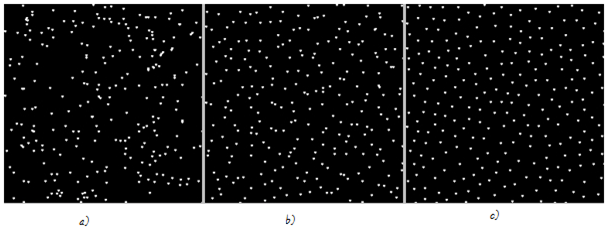
\includegraphics[width=0.5\textwidth]{./Cap2_videomapping/malla-poisson.png}
  \caption{a) Posición $x$ e $y$ generadas aleatoriamente. b) Imagen dividida en celdas. Puntos aleatorios generados en cada celda. c) Muestreo \emph{Poisson-disk} en dos dimensiones.}
  \label{fig:Mesh-Poisson}
\end{figure}

En líneas generales, este algoritmo genera puntos alrededor de los ya existentes en la muestra y valida si pueden ser agregados al conjunto final en caso de no violar la regla de la mínima distancia a los vecinos. Se genera una grilla en dos o tres dimensiones, dependiendo del escenario de aplicación, en la cuál cada celda contendrá al final del proceso a lo sumo un punto. Una grilla adicional es utilizada para realizar búsquedas rápidas y dos conjuntos de puntos son mantenidos durante el procesamiento para poder diferenciar los que han sido generados y los que aún necesitan procesamiento.
La implementación realizada en \emph{VcgLib} recibe tres parámetros:
\begin{itemize}
  \item 1) La cantidad de puntos en la muestra. En este caso el radio de cercanía es calculado en base a este parámetro.
  \item 2) El radio, que es a su vez utilizado para calcular el tamaño de la muestra óptimo en base a la malla inicial.
  \item 3) Sub muestreo: indica si la muestra de Poisson es un subconjunto de la muestra inicial o si se deberán generar nuevos puntos aleatoriamente.
\end{itemize}

\subsubsection{Reconstrucción de normales}

Este algoritmo computa las normales en cada elemento de un conjunto de puntos sin la necesidad de explorar la conectividad de los triángulos. Por ello es muy útil para objetos tridimensionales sin información de caras.
Se detalla un pseudo-código del método:

%Figura: planos tangentes%

\paragraph{Paso 1: identificar los planos tangentes para aproximar localmente la superficie y estimar así los vectores normales.}
Para cada vértice:
  \begin{itemize}
    \item Calcular el centro geométrico del plano tangente en el punto como el promedio de los $K$ puntos más cercanos.
    \item Calcular la normal asociada al centro geométrico. Se utiliza la matriz de covarianza en el punto, contemplando los mismos $K$ vecinos más cercanos de la muestra y los valores y vectores propios de la matriz de covarianza. Finalmente, ordenando los vectores propios, la estimación del vector perpendicular corresponde al vector propio de menor valor. Este método es conocido como \emph{Principal Component Analysis (PCA)}\footnote{PCA}.
  \end{itemize}

\paragraph{Paso 2: construir un grafo en donde cada punto está conectado a los $K$ vecinos más cercanos (grafo de Riemannian)}
Se crea un grafo en cuyos nodos se guardan todas las aristas incidentes a los $K$ vecinos más cercanos. A cada arista se le asigna un peso igual al valor absoluto del producto escalar de la normal en el punto con la normal en cada uno de los $K$ vecinos:
   $$fabs(nodoActual->normal . K\_Vecinos[n]->normal)$$
\paragraph{Paso 3: calcular el árbol de expansión mínimo sobre el grafo de Riemannian y recorrerlo para orientar las normales.}
Dado un grafo conexo, no dirigido, con sus aristas con un peso asignado, se llama árbol de expansión mínimo al sub-grafo con forma de árbol que conecta todos los nodos con un peso total mínimo conteniendo todos los nodos del grafo inicial. El grafo de entrada es el construido en el paso anterior y se utiliza el algoritmo de Kruskal\footnote{Kruskal}, uno de los varios algoritmos que resuelven el problema de encontrar un árbol de expansión mínima de un grafo.
Una vez construido el árbol de expansión, lo único que se hace es recorrerlo en orden e invertir el sentido de los vectores normales en caso de ser necesario. La condición para efectuar dicha corrección se basa en el ángulo del nodo siendo inspeccionado en comparación a todas las direcciones de las normales de los vecinos conectados a dicho nodo.

\subsubsection{Reconstrucción de malla de Poisson}

Finalmente, para reconstruir la malla a partir de la nube de puntos y sus normales, se utiliza el algoritmo de reconstrucción de Poisson.
Se computa una función indicadora $\chi$ definida de la siguiente forma:
%Se computa una función indicadora $\chi$ en tres dimensiones definida de la siguiente forma:%

$$
\left\{ \begin{array}{rl}
 \chi = 1 & \mbox{ si puntos dentro del modelo} \\
 \chi = 0 & \mbox{ si puntos fuera del modelo}
       \end{array} \right.
$$

Luego, se obtiene una reconstrucción de la superficie mediante la extracción de la superficie de nivel en 3 dimensiones\footnote{ISO-surface} al nivel apropiado.
La estrategia se basa en la estrecha relación que hay entre los puntos de la muestra, orientados por sus normales, y la función indicadora de la muestra. Específicamente el gradiente de la función indicadora es un espacio de vectores, de valor nulo en todo el espacio excepto en puntos cercanos a la superficie, donde son iguales al vector normal a ella.
Es por eso que puntos orientados pueden ser vistos como muestras del gradiente de la función indicadora del modelo tridimensional en cuestión y es por este mismo motivo que el problema de reconstrucción de una malla puede ser visto como un problema de Poisson estándar, es decir, computar la función escalar $F$ cuya divergencia del gradiente\footnote{Laplaciano} se iguala a la divergencia del espacio de vectores de las normales.

